\documentclass[a4paper,10pt]{article}
\usepackage[utf8]{inputenc}
\usepackage[T1]{fontenc}
\usepackage{lmodern}	
\usepackage[italian]{babel}

\usepackage{amsmath}
\usepackage{amsfonts}
\usepackage{amssymb}
\usepackage{bm}

\usepackage{graphicx}
\usepackage[dvipsnames]{xcolor}  %colori
\usepackage{pgf}
\usepackage{tikz}
\usetikzlibrary{arrows,shapes,snakes,automata,backgrounds,petri}	% Finite States Machine

\usepackage[left=2cm,right=2cm,top=2cm,bottom=2cm]{geometry}
\geometry{a4paper}

\usepackage{verbatim}

\usepackage{booktabs}
\usepackage{subfig}
\usepackage{float}

\usepackage[colorlinks=true, linkcolor=black, urlcolor=blue, citecolor=darkgray, filecolor=darkgray]{hyperref}   %per gli hyperlink
\usepackage[italian, sort, noabbrev, capitalise]{cleveref}
\usepackage[bottom]{footmisc}

\usepackage[cdot, thickqspace, squaren]{SIunits}
% macro
\def\code#1{\texttt{#1}}

\title{Esercitazione 13: Macchine a Stati Finiti: semaforo}
\author{Gruppo BL \\ Candido Alessandro, Luzio Andrea, Mazziotti Fabrizio}

\begin{document}

\maketitle

\section{Scopo e Strumentazione}
Lo scopo dell'esercitazione è la progettazione ed implementazione di un circuito che gestisce un semaforo come applicazione del concetto di una macchina a stati finiti (FSM).
\newline

\noindent La strumentazione è quella solitamente presente sul banco di lavoro, e inoltre si è usato:
\begin{itemize}
	\item 2 Integrati 7474 – 2 FF di tipo D;
	\item 1 Integrato 7400 – 4 Porte NAND;
	\item 1 Integrato 7408 – 4 Porte AND;
	\item 1 Integrato 7432 – 4 Porte OR;
	\item 3 LED: Verde, Rosso, Giallo;
	\item 1 Switch 4 bit.
\end{itemize}

\subsection{Specifiche}

Si riportano le specifiche del progetto:
\newline

\noindent Il semaforo può avere due modalità di funzionamento: “ABILITATO” o “DISABILITATO”.
\begin{itemize}
	\item 
	Nella modalità ABILITATO la sequenza degli stati, ripetuta ciclicamente, deve essere:
	
	\qquad LED Verde acceso $ \bm{\longrightarrow} $ LED Verde e Giallo acceso $ \bm{\longrightarrow} $ LED Rosso acceso
	
	\item Nella modalità DISABILITATO i led Verde e Rosso sono spenti ed il led Giallo lampeggia.
\end{itemize}
Tutti gli stati devono durare 1 impulso di clock. La modalità di funzionamento viene determinata tramite un interruttore che genera il segale di abilitazione (“E”=enable).

Si può scegliere se il segnale E sia attivo alto oppure attivo basso, ma fare attenzione ad essere consistenti nella definizione e nella analisi.

\section{Progettazione}

Si è scelto di implementare direttamente il semaforo con enable, in quanto è stato realizzato mantenendo la struttura fondamentale del caso abilitato (cioè apportando modifiche quanto più possibile leggere), la progettazione è avvenuta comunque in due fasi, che si procede ad illustrare.

\subsection{Semaforo nello stato abilitato}

In assenza di enable non ci sono ingressi, e il comportamento richiesto è la generazione in uscita di una sequenza di periodo $ 3 $, in cui ogni step duri un ciclo di clock.

Non c'è allora differenza tra una macchina di Mealy e una di Moore, e le uscite saranno funzione dello stato. Si è quindi deciso di codificare i $ 3 $ stati necessari usando $ 2 $ bit (cioè due flip flop). 

Si avrà quindi uno stato in eccesso, che non rientra nel ciclo. Per far sì che il circuito funzioni correttamente esso deve transire verso uno dei $ 3 $ stati permessi, in modo che in qualunque stato si trovi il flip flop all'accensione esso sia, già al secondo step, in uno dei tre stati permessi, e da lì continui a ciclare come stabilito.

Si riporta quindi in \cref{fig:wEN} il comportamento descritto, dove lo stato proibito è rappresentato con X.

\begin{figure}[H]
	\centering
	\begin{tikzpicture}[->,>=stealth',shorten >=1pt,auto,node distance=2.8cm,
thick]
\tikzstyle{every state}=[fill=none,draw=black,text=black]

\begin{scope}

\node[state]		 (A)              {R};	%$0-1$
\node[state]         (B) [below of=A] {V};	%$0-0$
\node[state]         (C) [below of=B] {VG};	%$1-0$
\node[state]         (D) [right of=B] {X};	%$1-1$

\path 	
(A) edge					node {}		(B)
(B) edge					node {} 	(C)
(C) edge [bend left]		node {} 	(A)
(D) edge [bend right=60]	node {} 	(A);

\end{scope}

%\begin{scope}[xshift=9cm]
%
%\node[state]		 (A')             	 	{R};	%$0-1$
%\node[state]         (B') [below of=A'] 	{V};	%$0-0$
%\node[state]         (C') [below of=B'] 	{VG};	%$1-0$
%\node[state]         (D') [right of=B'] 	{X};	%$1-1$
%
%\path 	
%(A') edge					node {}		(B')
%(B') edge					node {} 	(C')
%(C') edge [bend left]		node {} 	(A')
%(D') edge [bend right=60]	node {} 	(A');
%
%\path[dashed,draw=black!40]	
%(A') edge [bend left=70]		node {}		(C')
%(B') edge [bend left=50]		node {}		(C')
%(C') edge [bend left=70]		node {} 	(A')
%(D') edge [bend left]			node {} 	(A');
%
%\end{scope}
%
%\draw [-to,thick,snake=snake,segment amplitude=.4mm,segment length=2mm,line after snake=1mm,black!60]
%([xshift=1.3cm]D -| D) -- ([xshift=-2.7cm]B' -| A')
%node [above=1mm,midway,text width=3cm,text centered,black]
%{\Large Enable};

%\begin{pgfonlayer}{background}
%\filldraw [line width=0.15mm,join=round,white,draw=black,rounded corners]
%([xshift=-1cm,yshift=2mm]A.north -| B.west) rectangle ([xshift=2mm,yshift=-2mm]C.south -| D.east);
%%([xshift=-1.7cm,yshift=2mm]A'.north -| B'.west) rectangle ([xshift=2mm,yshift=-2mm]C'.south -| D'.east);
%\end{pgfonlayer}
\end{tikzpicture}
	\caption{Macchina a stati finiti per il caso di semaforo abilitato}
	\label{fig:wEN}
\end{figure}

Gli altri stati sono già stati indicati con le denominazioni relative alle uscite del circuito:
\begin{itemize}
	\item R è lo stato in cui l'uscita è costituita dal solo LED rosso acceso;
	\item V è lo stato in cui l'uscita è costituita dal solo LED verde acceso;
	\item VG è lo stato in cui l'uscita è costituita dal solo LED rosso spento, cioè i LED verde e giallo accesi contemporaneamente.
\end{itemize}
Lo schema riprodotto in \cref{fig:wEN} è quasi del tutto generale, a meno di un dettaglio: non è rilevante che la transizine dallo stato proibito sia X$ \rightarrow $R, ma è sufficiente qualunque stato permesso.
Quello riprodotto è quello che è stato scelto per il circuito implementato.

\paragraph{Codifica degli stati} Si è scelto di applicare la seguente codifica:
\begin{itemize}
	\item $ 1-1 $ stato proibito;
	\item $ 0-1 $ lo stato R;
	\item $ 1-0 $ lo stato VG;
	\item $ 0-0 $ lo stato V.
\end{itemize}
I motivi per la scelta della precedente codifica sono i seguenti:
\begin{enumerate}
	\item Invertire $ 1 $ e $ 0 $ in tutte le occorrenze è indifferente a livello di codifica, perché dai flip flop sono disponibili in uscita sia i valori memorizzati che gli stessi negati, per cui non c'è bisogno di ulteriori porte NOT in alcun caso;
	\item I LED rosso e verde non sono mai accesi contemporaneamente: si è quindi scelto di identificare le due possibili uscite di un bit (il secondo) una con l'accensione del verde e l'altra con quella del rosso;
	\item Il rosso è acceso in un solo stato durante il ciclo, quindi lo stato proibito deve coincidere con uno dei due in cui sia acceso il rosso;
	\item Si identifica una delle uscite dell'altro bit con il giallo, in modo da minimizzare la logica che genera l'output (non essendoci è minima necessariamente), in questo modo gli stati dell'altro bit indicheranno se il LED giallo sia acceso o spento\footnote{\`E stato pensato in questo modo anche per facilitare la realizzazione dello stato DISABILITATO.}. A questo punto gli stati sono identificati quindi con i seguenti valori per le uscite:
	\begin{itemize}
		\item giallo acceso $ - $ rosso;
		\item giallo spento $ - $ rosso;
		\item giallo acceso $ - $ verde;
		\item giallo spento $ - $ verde;
	\end{itemize}
\end{enumerate}
Si è quindi scelto che i due bit siano quindi del tutto indipendenti, e la codifica dovrà soddisfare questi requisiti. Le scelte residue sono quindi solo $ 2 $: se attribuire al verde il valore $ 0 $ o $ 1 $ del secondo bit, e al giallo il valore $ 0 $ o $ 1 $ del primo.

Per il punto $ 1 $ del precedente elenco l'unica cosa rilevante, a livello di uscite, è la codifica \textit{relativa} per cui la scelta fondamentale è se fissare lo stato VG\footnote{Si è detto al punto $ 4 $ che gli stati sono identificati con le uscite.} in uno stato in cui i due flip flop hanno lo stesso valore oppure diverso.

\subparagraph{Osservazione} Si è detto che la codifica assoluta non è rilevante, e questo è vero in teoria, poiché negando i valori di tutti gli stati e tutte le uscite si ottiene esattamente lo stesso circuito, sostituendo però le porte AND con porte OR e viceversa. In laboratorio si avevano a disposizione tante porte AND quante OR, si avevano però porte NAND, ma non porte NOR.

Per questo motivo la situazione è leggermente asimmetrica, e anche una delle due codifiche \textit{assolute} è facorita.

\subsubsection{Tabelle di verità}
Si sono realizzate le tabelle di verità del circuito rappresentato in \cref{fig:circuit}; nella \tablename{~\ref{tab:sem1}} sono rappresentate le transizioni di stato e le uscite in relazioni agli ingressi del circuito quando il semaforo è abilitato (Enable = 1).


\begin{table}[H]
	\centering
	\begin{tabular}{c|cc|cc|ccc|ccc}
		\hline
		$Enable$ & $Q1_n$ &	$Q2_n$ & $Q1_{n+1}$ & $Q2_{n+1}$ & $V_n$ & $G_n$ & $R_n$ & $V_{n+1}$ & $G_{n+1}$ & $R_{n+1}$ \\
		\hline
		1 & 1 & 1 & 0 & X & X & X & X & X & X & X \\
		\hline
		1 & 0 & 1 & 0 & 0 & 0 & 0 & 1 & 1 & 0 & 0 \\
		1 & 0 & 0 & 1 & 0 & 1 & 0 & 0 & 1 & 1 & 0 \\
		1 & 1 & 0 & 0 & 1 & 1 & 1 & 0 & 0 & 0 & 1 \\
		\hline
	\end{tabular}
	\caption[Semaforo Abilitato]{Tabella di verità del circuito in esame quando il semaforo è abilitato\footnotemark.}
	\label{tab:sem1}
\end{table}
\footnotetext{Gli stati contrassegnati con le X sono stati Don't Care.}

\begin{itemize}
	\item Le variabili $Q1_n$, $Q2_n$ rappresentano gli stati n-esimi dei due FF;
	\item le variabili $Q1_{n+1}$, $Q2_{n+1}$ sono gli stati (n+1)-esimi dei due FF;
	\item gli stati $V_n$,$G_n$,$R_n$ rappresentano le uscite n-esime, visualizzate sui LED (rispettivamente il led Verde, Giallo, Rosso);
	\item gli stati $V_{n+1}$,$G_{n+1}$,$R_{n+1}$ rappresentano le uscite (n+1)-esime, visualizzate sui LED;
\end{itemize}
Gli stati contrassegnati con una 'X' sono stati don't care, e sono posti in corrispondenza dello stato dei FF indesiderato, poiché per esso l'unica azione rilevante è la transizione su un altro stato, che p stata imposta fissato $ Q1_{n+1} = 0 $.

Per come è stato costruito il circuito lo stato indesiderato ($Q1_n$ = $Q2_n$ = 1) porta a sostituire le X con quanto riportato in \tablename{~\ref{tab:inde}}, come affermato nella sezione precedente.

\begin{table}[H]
	\centering
	\begin{tabular}{c|cc|cc|ccc|ccc}
		\hline
		$Enable$ & $Q1_n$ &	$Q2_n$ & $Q1_{n+1}$ & $Q2_{n+1}$ & $V_n$ & $G_n$ & $R_n$ & $V_{n+1}$ & $G_{n+1}$ & $R_{n+1}$ \\
		\hline
		1 & 1 & 1 & 0 & 1 & 0 &  1 & 1 & 0 & 0 & 1  \\
		\hline
	\end{tabular}
	\caption{Tabella di verità per lo stato indesiderato quando il semaforo è abilitato.}
	\label{tab:inde}
\end{table}
%
%Quindi come si può vedere dalle due tabelle, se si capita (all'accensione del circuito) nello stato indesiderato, il led giallo e rosso sono accesi contemporaneamente. Al colpo successivo di clock le uscite dei FF cadono negli stati in corrispondenza dei quali solo il led Rosso è acceso. Da questo momento in poi si alternano gli stati Rosso, Verde, Verde-Giallo e non si può più ricadere nello stato indesiderato.

\paragraph{Funzioni combinatorie}
Qui di seguito si riportano l'espressione degli stati in uscita agli FF e le uscite del circuito in funzione di $Q1_n$, $Q2_n$ e dell'enable (EN) quando il semaforo è abilitato (al posto dei don't care, per definire le funzioni, è stata utilizzata la \cref{tab:inde})\footnote{In questo caso EN = 1 sempre, quindi l'Enable è superfluo ogni volta che è in un AND.}
\begin{itemize}
\item $Q1_{n+1}$ =$ EN \cdot \bar{Q1}_n \cdot \bar{Q2}_n $ = $\bar{Q1}_n \cdot \bar{Q2}_n $
\item $Q2_{n+1}$ = $EN \cdot Q1_n$ = $Q1_n$ 
\item $V_{n}$ = $EN \cdot \bar{Q2}_n$ = $\bar{Q2}_n$
\item $G_{n}$ = $ EN \cdot Q1_n$ = $Q1_n$ 
\item $R_{n}$ = $EN \cdot Q2_n$ = $Q2_n$ 
\end{itemize}


\subsection{Semaforo completo con lampeggiante}

Si è progettato il semaforo con enable seguendo i seguenti criteri:
\begin{enumerate}
	\item Nel caso precedente lo stato cui è associato il giallo è realizzato dipende da un singolo flip flop, per cui è sufficiente
	\begin{itemize}
		\item porre questo FF oscillante quando EN $ = 0 $;
		\item imporre che quando  EN $ = 0 $ i LED verde e rosso siano spenti, a prescindere dallo stato dei registri.
	\end{itemize}
	\item si cerca di minimizzare il numero di transizioni da cambiare rispetto al caso precedente quando EN $ = 0 $.
\end{enumerate}

\begin{figure}[H]
	\centering
	\begin{tikzpicture}[->,>=stealth',shorten >=1pt,auto,node distance=2.8cm,
thick]
\tikzstyle{every state}=[fill=none,draw=black,text=black]

\begin{scope}

\node[state]		 (A)              {R};	%$0-1$
\node[state]         (B) [below of=A] {V};	%$0-0$
\node[state]         (C) [below of=B] {VG};	%$1-0$
\node[state]         (D) [right of=B] {X};	%$1-1$

\path 	
(A) edge					node {}		(B)
(B) edge					node {} 	(C)
(C) edge [bend left]		node {} 	(A)
(D) edge [bend right=60]	node {} 	(A);

\end{scope}

\begin{scope}[xshift=9cm]

\node[state]		 (A')             	 	{R};	%$0-1$
\node[state]         (B') [below of=A'] 	{V};	%$0-0$
\node[state]         (C') [below of=B'] 	{VG};	%$1-0$
\node[state]         (D') [right of=B'] 	{X};	%$1-1$

\path 	
(A') edge					node {}		(B')
(B') edge					node {} 	(C')
(C') edge [bend left]		node {} 	(A')
(D') edge [bend right=60]	node {} 	(A');

\path[dashed,draw=black!40]	
(A') edge [bend left=70]		node {}		(C')
(B') edge [bend left=50]		node {}		(C')
(C') edge [bend left=70]		node {} 	(A')
(D') edge [bend left]			node {} 	(A');

\end{scope}

\draw [-to,thick,snake=snake,segment amplitude=.4mm,segment length=2mm,line after snake=1mm,black!60]
([xshift=1.3cm]D -| D) -- ([xshift=-2.7cm]B' -| A')
node [above=1mm,midway,text width=3cm,text centered,black]
{\Large Enable};

%\begin{pgfonlayer}{background}
%\filldraw [line width=0.15mm,join=round,white,draw=black,rounded corners]
%([xshift=-1cm,yshift=2mm]A.north -| B.west) rectangle ([xshift=2mm,yshift=-2mm]C.south -| D.east)
%([xshift=-1.7cm,yshift=2mm]A'.north -| B'.west) rectangle ([xshift=2mm,yshift=-2mm]C'.south -| D'.east);
%\end{pgfonlayer}
\end{tikzpicture}
	\caption{Macchine a stati finiti per i due casi: con e senza enable}
	\label{fig:EN}
\end{figure}

Si sono quindi fissate le transizioni come mostrato in \cref{fig:EN}, in cui nello schema di destra sono rappresentate con una linea continua le transizioni per EN $ = 1 $ e con una linea tratteggiata quelle per EN $ = 0 $.
\newline

Si noti che per passare da un caso all'altro è stato sufficiente cambiare un'unica transizione, imponendo di fatto che ci siano due stati proibiti, e che i due stati permessi ciclino fra di loro (di cui ovviamente uno avrà il giallo acceso, VG, e l'altro spento).
\newline

Non si procede a illustrare una nuova codifica, perché da quanto si è affermato fin qui è evidente che si è scelto di mantenere la stessa codifica del caso precedente.

\paragraph{Macchina di Mealy/Moore} Si è scelto di realizzare una macchina di Mealy, come mostrato in \cref{fig:circuit}; si nota che la realizzazione di una macchina di Moore prevederebbe la sola sincronizzazione dell'enable, ponendo un flip flop che riceva EN come dato e lo comunichi al resto del circuito attraverso la sua uscita Q, senza che sia necessaria l'aggiunta di ulteriore logica (in questo caso gli stati considerati sarebbero $ 8 $, dato che si inserirebbe un ulteriore bit, e quindi sarebbero in tutto $ 3 $, ma sostanzialmente coincide con quanto è stato fatto).

\subsubsection{Tabelle di verità}

Nella \tablename{~\ref{tab:lampe}} sono rappresentate le transizioni di stato e le uscite in relazioni agli ingressi del circuito quando il semaforo è disabilitato (Enable = 0). Le varie variabili utilizzate della tabella hanno la stessa definizione del caso del semaforo abilitato.
 
 \begin{table}[H]
	\centering
	\begin{tabular}{c|cc|cc|ccc|ccc}
	\hline
	Enable & $Q1_n$ & $Q2_n$ & $Q1_{n+1}$ & $Q2_{n+1}$ & $V_n$ & $G_n$ & $R_n$ & $V_{n+1}$ & $G_{n+1}$ & $R_{n+1}$ \\
	\hline
	0 & 1 & 1 & 0 & 1 & 0 & 1 & 0 & 0 & 0 & 0 \\
	0 & 0 & 1 & 1 & 0 & 0 & 0 & 0 & 0 & 1 & 0 \\
	0 & 0 & 0 & 1 & 0 & 0 & 0 & 0 & 0 & 1 & 0 \\
	0 & 1 & 0 & 0 & 1 & 0 & 1 & 0 & 0 & 0 & 0 \\
	\hline
		\end{tabular}
	\caption{Tabella di verità del circuito in esame quando il semaforo è disabilitato.}
	\label{tab:lampe}
\end{table}

Come si può vedere dalla tabella, qui non ci sono stati non permessi, poiché quando l'enable è 0, automaticamente il Led Rosso e Verde sono spenti per via delle due porte AND ai loro ingressi (vedere \cref{fig:circuit}). In ogni caso quindi il Led Giallo è acceso o spento e inverte il suo stato a ogni colpo di clock, come voluto.

\paragraph{Funzioni combinatorie}
Qui di seguito si riportano l'espressione degli stati in uscita agli FF e le uscite del circuito in funzione di $Q1_n$, $Q2_n$ e dell'enable (EN) quando il semaforo è disabilitato:
\begin{itemize}
\item $Q1_{n+1}$ = $\bar{EN} \cdot \bar{Q1_n} \cdot Q2_n + \bar{EN} \cdot \bar{Q1_n} \cdot \bar{Q2_n} = \bar{Q1_n}$
\item $Q2_{n+1}$ = $\bar{EN} \cdot Q1_n$ = $Q1_n$
\item $V_{n}$ = 0 (funzione nulla)
\item $G_{n}$ = $\bar{EN} \cdot Q1_n$ = $Q1_n$
\item $R_{n}$ = 0 (funzione nulla)
\end{itemize}

\section{Implementazione}

Si riporta in \cref{fig:circuit} il circuito realizzato.
Relativamente ai flip flop: i pin inferiori rappresentano gli ingressi di PRESET e CLEAR, che sono stati collegati all'alimentazione per evitare reset o clear spurii.

\begin{figure}[H]
	\centering
	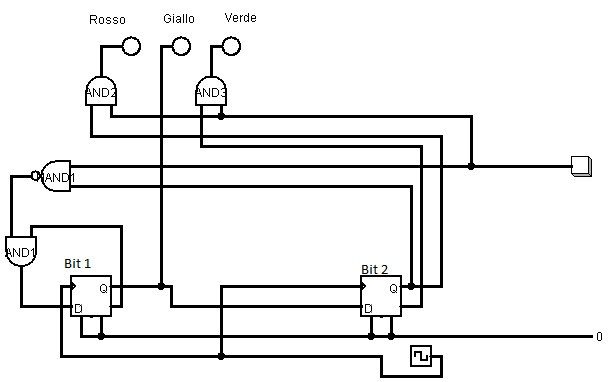
\includegraphics[width=0.7\textwidth]{../grafici/circuito1.png}
	\caption{Circuito realizzato per il semaforo completo}
	\label{fig:circuit}
\end{figure}


Si è cercato di ottimizzare la rete combinatoria cercando di minimizzare in primo luogo il numero di integrati da usare, in secondo luogo il numero di porte da adoperare. L'approccio logico adottato è abbastanza semplice: si sono individuate le due modalità di funzionamento (enabled=\code{HIGH} e enabled=\code{LOW}) e si sono ottimizzati i relativi circuiti. 
I circuiti ottenuti sono disegnati in \cref{fig:enabled} e \cref{fig:disabled}.



Come si può vedere in \cref{fig:disabled} la logica necessaria per le transizioni nello stato enabled=\code{LOW} è necessariamente la minima. Di fatto basta mandare l'uscita negata all'ingresso.


Per lo stato enabled=\code{HIGH} si deve usare almeno una porta (un AND). 
\'E una mera verifica la tabella di verità \cref{tab:sem1} (con i don't care sostituiti con 1).



\begin{figure}[H]
	\centering
	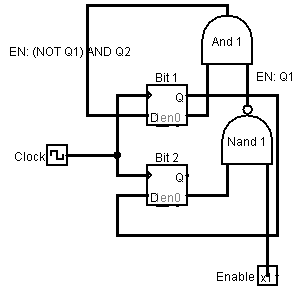
\includegraphics[width=0.4\textwidth]{../grafici/enabled1.png}
	\caption{Idealizzazione delle funzione di trasferimento con circuito enabled=\code{HIGH}}
	\label{fig:enabled}
\end{figure}


\begin{figure}[H]
	\centering
	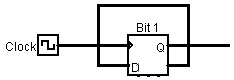
\includegraphics[width=0.4\textwidth]{../grafici/disabled1.png}
	\caption{Idealizzazione delle funzione di trasferimento con circuito enabled=\code{LOW}}
	\label{fig:disabled}
\end{figure}

A questo punto la sfida è fare in modo che l'enable permetta la transizione fra le due modalità di funzionamento, e, nello stesso tempo, impedisca che i segnali presenti sul secondo flip-flop vengano mandati ai led Rosso e Verde (che devono stare spenti quando il dispositivo è disabilitato).

Per quanto riguarda la logica di trasferimento si può fare riferimento a \cref{fig:solologica}: si è interposta prima della AND1 un NAND (NAND1) (con il segnale di ENABLE). Questo, quando il dispositivo è abilitato, si comporta come un mero NOT. E' dunque stato sufficiente collegare l'altro ingresso del NAND con $\bar{Q}$ per ristabilire il corretto funzionamento della rete di transizione quando enabled=\code{HIGH}.

Si nota che quando ENABLED è invece \code{LOW} l'output della NAND è \code{HIGH} quindi anche il comportamento nella configurazione disabilitata è quello corretto.

Per quanto riguarda i led si è dovuti ricorrere a due AND con il segnale ENABLE: l'AND è l'unica porta fra quelle date a disposizione che nella modalità forzata ha l'uscita \code{LOW} (ovvero che possa essere forzata \code{LOW} da uno solo dei due ingressi, indipendentemente dall'altro\footnote{Sia il NAND che l'OR possono essere forzati \code{HIGH}, cosa inutile per il funzionamento del semaforo.}).

Non si sono cercate ulteriori ottimizzazioni poiché proprio quest'ultimo fatto forza ad usare almeno un AND. Chiaramente non è possibile costruire l'intero circuito utilizzando solamente AND \footnote{Si ricorda che la logica della AND è associativa, dunque l'unica scelta possibile rimanente sarebbe stata quali (non in che ordine) ingressi scegliere per la nostra porta fra Q1, Q2 (o i rispettivi negati) ed EN. Ma nessuna delle alternative porta alla funzione di trasmissione richiesta, dunque è necessario almeno un NAND.} 

\'E necessario spendere due parole per quanto riguarda quello che succede proprio quando EN cambia stato (il che, essendo esso asincorno, avverrà all' interno di un ciclo di clock). Se EN passa da \code{HIGH} a \code{LOW} non avviene nulla di dannoso: gli AND che controllano i led rosso e verde impediranno che essi siano accesi e il giallo continuerà a essere nello stato che aveva prima che EN fosse commutato. Poi inizierà la sua usuale oscillazione.

Se invece  EN passa dallo stato \code{LOW} a \code{HIGH} ci si può chiedere se sia visibile la condizione "vietata" 11, che sarebbe particolarmente fastidiosa in quanto permetterebbe al led rosso di essere acceso contemporaneamente al led giallo. Questo in effetti non accade perché quando EN era \code{LOW} lo stato del secondo bit è sempre opposto a quello del primo bit. Dunque se il primo bit è 1 il secondo è 0 e la configurazione "vietata" 11 è salta.





\begin{figure}[H]
	\centering
	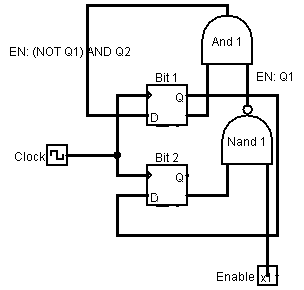
\includegraphics[width=0.4\textwidth]{../grafici/solologica1.png}
	\caption{Idealizzazione delle funzione di trasferimento con entrambi i valori di ENABLED. Per chiarezza si sono indicati i valori logici fondamentali nel caso ENABLED = \code{HIGH}}
	\label{fig:solologica}
\end{figure}


Infine si può notare che per rendere sincrono il dispositivo sarebbe bastato mettere un altro D letch nel canale del ENABLE. 


\section{Verifica del funzionamento}

Montato il circuito si è dunque verificato l'opportuno funzionamento dello stesso. Per fare ciò il clock è stato portato a qualche centinaio di Hz e si sono visualizzate le tracce con l'oscilloscopio.

Si sono ottenute le seguenti tracce:


\begin{figure}[H]
	\centering
	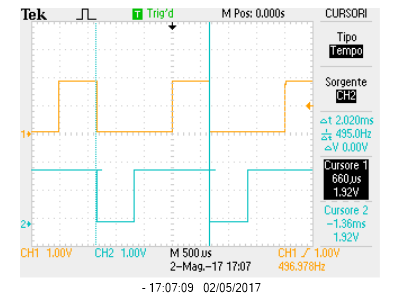
\includegraphics[width=0.4\textwidth]{../grafici/verde_giallo.png}
	\caption{Output del verde e del giallo con ENABLE = \code{HIGH} (modalità tre colori)}
	\label{fig:VGE}
\end{figure}

Come si vede in \cref{VGE} dapprima sia il segnale per il verde che quello per il giallo sono entrambi \code{LOW}, dopo un terzo del periodo (che dura tre cicli di clock) il verde diventa \code{HIGH} mentre il giallo rimane \code{LOW}, per l'ultimo terzo sono entrambi \code{HIGH}.



\begin{figure}[H]
	\centering
	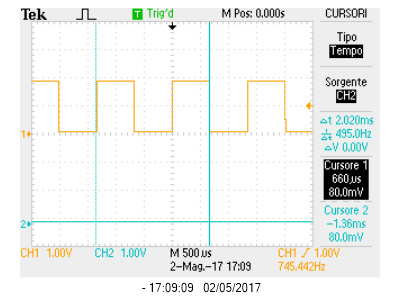
\includegraphics[width=0.4\textwidth]{../grafici/verde_gialloELOW.png}
	\caption{Output del verde (traccia azzurra) e del giallo con ENABLE=\code{LOW} (modalità due colori)}
	\label{fig:VGELOW}
\end{figure}

Come si vede in \cref{ELOW} anche in modalità lampeggiante il giallo è il verde negato. Qui il ciclo completo dura solo due clock.


\section{FSM in Software}

Si è semplicemente caricato il programma e verificato il funzionamento. Non aveva alcun senso fare altro per un semplice semaforo. E' un po come sparare col cannone su un coniglio...



\end{document}